\documentclass[border=4pt]{standalone}
\usepackage{adjustbox}
\usepackage{tikz}
\usetikzlibrary{positioning,arrows.meta,shapes.geometric}
\begin{document}
\begin{adjustbox}{max width=\textwidth}
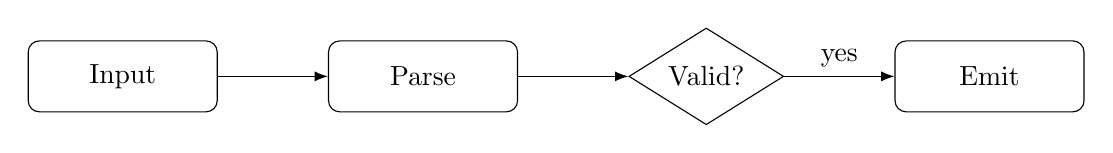
\begin{tikzpicture}[node distance=10mm and 14mm]
\node[draw, rounded corners, minimum width=24mm, minimum height=9mm] (input) {Input};
\node[draw, rounded corners, minimum width=24mm, minimum height=9mm, right=of input] (parse) {Parse};
\node[draw, diamond, aspect=1.6, minimum width=18mm, minimum height=12mm, right=of parse] (check) {Valid?};
\node[draw, rounded corners, minimum width=24mm, minimum height=9mm, right=of check] (emit) {Emit};
\draw[-{Latex}] (input) -- (parse);
\draw[-{Latex}] (parse) -- (check);
\draw[-{Latex}] (check) -- node[above] {yes} (emit);
\end{tikzpicture}
\end{adjustbox}
\end{document}
